%%%%%%%%%%%%%%%%%%%%%%%%%%%%%%%%%%%%%%%%%%%%%%%%%%%%%%%%%%%%%%%%%%%%%
% LaTeX Template: Project Titlepage Modified (v 0.1) by rcx
%
% Original Source: http://www.howtotex.com
% Date: February 2014
% 
% This is a title page template which be used for articles & reports.
% 
% This is the modified version of the original Latex template from
% aforementioned website.
% 
%%%%%%%%%%%%%%%%%%%%%%%%%%%%%%%%%%%%%%%%%%%%%%%%%%%%%%%%%%%%%%%%%%%%%%

\documentclass[12pt]{article}
\usepackage[a4paper]{geometry}
\usepackage[myheadings]{fullpage}
\usepackage{fancyhdr}
\usepackage{lastpage}
\usepackage{graphicx, wrapfig, subcaption, setspace, booktabs}
\usepackage[T1]{fontenc}
\usepackage[font=small, labelfont=bf]{caption}
\usepackage{fourier}
\usepackage[protrusion=true, expansion=true]{microtype}
\usepackage[english]{babel}
\usepackage{sectsty}
\usepackage{url, lipsum}
\usepackage{tgbonum}
\usepackage{hyperref}
\usepackage{xcolor}
\usepackage{dirtytalk}
\graphicspath{ {images/} }
\usepackage{textcomp}

\newcommand{\HRule}[1]{\rule{\linewidth}{#1}}
\onehalfspacing
\setcounter{tocdepth}{5}
\setcounter{secnumdepth}{5}



%-------------------------------------------------------------------------------
% HEADER & FOOTER
%-------------------------------------------------------------------------------
%\pagestyle{fancy}
%\fancyhf{}
%\setlength\headheight{15pt}
%\fancyhead[L]{Student ID: 1034511}
%\fancyhead[R]{Anglia Ruskin University}
%\fancyfoot[R]{Page \thepage\ of \pageref{LastPage}}
%-------------------------------------------------------------------------------
% TITLE PAGE
%-------------------------------------------------------------------------------

\begin{document}
{\fontfamily{cmr}\selectfont
\title{ \normalsize \textsc{}
		\\ [2.0cm]
		\HRule{0.5pt} \\
		\LARGE \textbf{\uppercase{Machine Learning}
		\HRule{2pt} \\ [0.5cm]
		\normalsize \today \vspace*{5\baselineskip}}
		}

\date{}

\author{
		Dhwani Agarwal\\ 
		ID : 171081018 \\
		Veermata Jijabai Technological Institute\\
		Department: Information Technology\\
		Professor: Pranav Nerurkar}

\maketitle
\newpage
\tableofcontents
\listoffigures
\newpage

%-------------------------------------------------------------------------------
% Section title formatting
\sectionfont{\scshape}
%-------------------------------------------------------------------------------

%-------------------------------------------------------------------------------
% BODY
%-------------------------------------------------------------------------------

\section{INTRODUCTION TO MACHINE LEARNING}
%\begin{enumerate}
    The term Machine Learning was coined by Arthur Samuel in 1959, an American pioneer in the field of computer gaming and artificial intelligence and stated that \say{it gives computers the ability to learn without being explicitly programmed.}
And in 1997, Tom Mitchell gave a \say{well-posed} mathematical and relational definition that \say{A computer program is said to learn from experience E with respect to some task T and some performance measure P, if its performance on T, as measured by P, improves with experience E.}

    To understand Machine Learning in layman terms, consider you are trying to toss a paper to a dustbin. After first attempt, you realize that you have put too much force in it. After second attempt, you realize you are closer to target but you need to increase your throw angle. What is happening here is basically after every throw we are learning something and improving the end result. We are programmed to learn from our experience.

This implies that the tasks in which machine learning is concerned offers a fundamentally operational definition rather than defining the field in cognitive terms. The question \SAY{Can machines think?} is replaced with the question \say{Can machines do what we (as thinking entities) can do?}
Within the field of data analytics, machine learning is used to devise complex models and algorithms that lend themselves to prediction; in commercial use, this is known as predictive analytics. These analytical models allow researchers, data scientists, engineers, and analysts to \say{produce reliable, repeatable decisions and results} and uncover \say{hidden insights} through learning from historical relationships and trends in the data set(input).

\end{enumerate}
%\newpage
%\section{Getting Started}
%\input{getstart.tex}
The term Machine Learning was coined by Arthur Samuel in 1959, an American pioneer in the field of computer gaming and artificial intelligence and stated that \say{it gives computers the ability to learn without being explicitly programmed.}
And in 1997, Tom Mitchell gave a \say{well-posed} mathematical and relational definition that \say{A computer program is said to learn from experience E with respect to some task T and some performance measure P, if its performance on T, as measured by P, improves with experience E.}

To understand Machine Learning in layman terms, consider you are trying to toss a paper to a dustbin. After first attempt, you realize that you have put too much force in it. After second attempt, you realize you are closer to target but you need to increase your throw angle\cite{g}. What is happening here is basically after every throw we are learning something and improving the end result. We are programmed to learn from our experience.

This implies that the tasks in which machine learning is concerned offers a fundamentally operational definition rather than defining the field in cognitive terms. The question \say{Can machines think?} is replaced with the question \say{Can machines do what we (as thinking entities) can do?}
Within the field of data analytics, machine learning is used to devise complex models and algorithms that lend themselves to prediction; in commercial use, this is known as predictive analytics. These analytical models allow researchers, data scientists, engineers, and analysts to \say{produce reliable, repeatable decisions and results} and uncover \say{hidden insights} through learning from historical relationships and trends in the data set(input).
\begin{figure}
    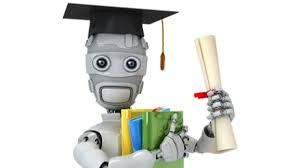
\includegraphics{ml.jpeg}
    \centering
    \caption{Machine Learning}
    \source{Source: https://www.expertsystem.com/machine-learning-definition/}
\end{figure}
\section{HISTORY }
%\begin{enumerate}
    As a scientific endeavour, machine learning grew out of the quest for artificial intelligence. Already in the early days of AI as an academic discipline, some researchers were interested in having machines learn from data. They attempted to approach the problem with various symbolic methods, as well as what were then termed \say{neural networks}; these were mostly perceptrons and other models that were later found to be reinventions of the generalized linear models of statistics.Probabilistic reasoning was also employed, especially in automated medical diagnosis.Machine learning, reorganized as a separate field, started to flourish in the 1990s. The field changed its goal from achieving artificial intelligence to tackling solvable problems of a practical nature. It shifted focus away from the symbolic approaches it had inherited from AI, and toward methods and models borrowed from statistics and probability theory.It also benefited from the increasing availability of digitized information, and the ability to distribute it via the Internet. 
    
    \subsection{RELATION TO DATA MINING}
\end{enumerate}
As a scientific endeavour, machine learning grew out of the quest for artificial intelligence. Already in the early days of AI as an academic discipline, some researchers were interested in having machines learn from data. They attempted to approach the problem with various symbolic methods, as well as what were then termed \say{neural networks}; these were mostly perceptrons and other models that were later found to be reinventions of the generalized linear models of statistics.Probabilistic reasoning was also employed, especially in automated medical diagnosis.Machine learning, reorganized as a separate field, started to flourish in the 1990s. The field changed its goal from achieving artificial intelligence to tackling solvable problems of a practical nature. It shifted focus away from the symbolic approaches it had inherited from AI, and toward methods and models borrowed from statistics and probability theory.It also benefited from the increasing availability of digitized information, and the ability to distribute it via the Internet. 
    
  %  \subsection{Relation to Data Mining}
%Machine learning and data mining often employ the same methods and overlap significantly, but while machine learning focuses on prediction, based on known properties learned from the training data, data mining focuses on the discovery of (previously) unknown properties in the data (this is the analysis step of knowledge discovery in databases). Data mining uses many machine learning methods, but with different goals; on the other hand, machine learning also employs data mining methods as "unsupervised learning" or as a preprocessing step to improve learner accuracy. Much of the confusion between these two research communities (which do often have separate conferences and separate journals, ECML PKDD being a major exception) comes from the basic assumptions they work with: in machine learning, performance is usually evaluated with respect to the ability to reproduce known knowledge, while in knowledge discovery and data mining (KDD) the key task is the discovery of previously unknown knowledge. Evaluated with respect to known knowledge, an uninformed (unsupervised) method will easily be outperformed by other supervised methods, while in a typical KDD task, supervised methods cannot be used due to the unavailability of training data. 

%\subsection{Relation to Optimization}
%Machine learning also has intimate ties to optimization: many learning problems are formulated as minimization of some loss function on a training set of examples. Loss functions express the discrepancy between the predictions of the model being trained and the actual problem instances (for example, in classification, one wants to assign a label to instances, and models are trained to correctly predict the pre-assigned labels of a set of examples). The difference between the two fields arises from the goal of generalization: while optimization algorithms can minimize the loss on a training set, machine learning is concerned with minimizing the loss on unseen samples.

%\subsection{Relation to Statistics}
%Machine learning and statistics are closely related fields. The ideas of machine learning, from methodological principles to theoretical tools, have had a long pre-history in statistics. He also suggested the term data science as a placeholder to call the overall field.Leo Breiman distinguished two statistical modelling paradigms: data model and algorithmic model,wherein "algorithmic model" means more or less the machine learning algorithms like Random forest.Some statisticians have adopted methods from machine learning, leading to a combined field that they call statistical learning.

\section{CLASSIFICATION OF MACHINE LEARNING}
%\begin{enumerate}
    \item SMART: Specific, Measurable, Actionable, Realistic, Time-based.
    \item Ex. I will write 2 pages of my report by 1/30/19.
    \item Ex. I will gather feedback from 2 peers about my idea by 1/30/19. 
    \item Ex. I will research a new theory for 2 hours by 1/17/19. 
\end{enumerate}
Machine learning implementations are classified into three major categories, depending on the nature of the learning \say{signal} or \say{response} available to a learning system which are as follows:-
\subsection{Supervised Learning}
When an algorithm learns from example data and associated target responses that can consist of numeric values or string labels, such as classes or tags, in order to later predict the correct response when posed with new examples comes under the category of Supervised learning. This approach is indeed similar to human learning under the supervision of a teacher. The teacher provides good examples for the student to memorize, and the student then derives general rules from these specific examples.

\subsection{Unsupervised Learning}
Whereas when an algorithm learns from plain examples without any associated response, leaving to the algorithm to determine the data patterns on its own. This type of algorithm tends to restructure the data into something else, such as new features that may represent a class or a new series of un-correlated values. They are quite useful in providing humans with insights into the meaning of data and new useful inputs to supervised machine learning algorithms. As a kind of learning, it resembles the methods humans use to figure out that certain objects or events are from the same class, such as by observing the degree of similarity between objects. Some recommendation systems that you find on the web in the form of marketing automation are based on this type of learning.

\subsection{Reinforcement Learning}
When you present the algorithm with examples that lack labels, as in unsu-pervised learning. However, you can accompany an example with positive or negative feedback according to the solution the algorithm proposes comes under the category of Reinforcement learning, which is connected to applications for which the algorithm must make decisions (so the product is prescriptive, not just descriptive, as in unsupervised learning), and the decisions bear consequences. In the human world, it is just like learning by trial and error.
Errors help you learn because they have a penalty added (cost, loss of time, regret, pain, and so on), teaching you that a certain course of action is less likely to succeed than others. An interesting example of reinforcement learning occurs when computers learn to play video games by themselves.
In this case, an application presents the algorithm with examples of specific situations, such as having the gamer stuck in a maze while avoiding an enemy. The application lets the algorithm know the outcome of actions it takes, and learning occurs while trying to avoid what it discovers to be dan-gerous and to pursue survival. You can have a look at how the company Google DeepMind has created a reinforcement learning program that plays old Atari\textquotesingle s videogames. When watching the video, notice how the program is initially clumsy and unskilled but steadily improves with training until it becomes a champion.

\subsection{Semi Supervised Learning}
Where an incomplete training signal is given: a training set with some (often many) of the target outputs missing. There is a special case of this principle known as Transduction where the entire set of problem instances is known at learning time, except that part of the targets are missing.

\section{MACHINE LEARNING APPLICATIONS}
The other aspect for classifying learning systems is the area of application which gives a new dimension for machine learning\cite{t}. Below are areas to which various existing learning systems have been applied. They are:
\begin{enumerate}
\item Computer Programming
\item Game playing (chess, poker, and so on)
\item Image recognition, Speech recognition
\item Medical diagnosis
\item Agriculture, Physics
\item Email management, Robotics
\item Music
\item Mathematics
\item Natural Language Processing and many more.
\end{enumerate}

\section{EXAMPLES OF MACHINE LEARNING PROBLEMS}
There are many examples of machine learning problems. Some of them include :
\begin{enumerate}
\item Optical character recognition: categorize images of handwritten characters by the letters represented
\item Face detection: find faces in images (or indicate if a face is present)
\item Spam filtering: identify email messages as spam or non-spam
\item Topic spotting: categorize news articles (say) as to whether they are about politics, sports, entertainment, etc.
\item Spoken language understanding: within the context of a limited domain, determine the meaning of something uttered by a speaker to the extent that it can be classified into one of a fixed set of categories
\item Medical diagnosis: diagnose a patient as a sufferer or non-sufferer of some disease
\item Customer segmentation: predict, for instance, which customers will respond to a particular promotion
\item Fraud detection: identify credit card transactions (for instance) which may be fraudulent in nature
\item Weather prediction: predict, for instance, whether or not it will rain tomorrow
\end{enumerate}

%-------------------------------------------------------------------------------
% REFERENCES
%-------------------------------------------------------------------------------
\newpage
%\section*{References}

%[2]John W. Eaton, David Bateman, Sren Hauberg, Rik Wehbring (2015). GNU
%Octave version 4.0.0 manual: a high-level interactive language for numer-
%ical computations. Available: http://www.gnu.org/software/octave/doc/
%interpreter/. 
\begin{thebibliography}{9}
\bibitem{g} https://www.geeksforgeeks.org/introduction-machine-learning
\bibitem{t} https://www.topicsforseminar.com/2018/05/seminar-report-on-machine-learning.html?m=1
\end{thebibliography}
\end{document}

%-------------------------------------------------------------------------------
% SNIPPETS
%-------------------------------------------------------------------------------

%\begin{figure}[!ht]
%	\centering
%	\includegraphics[width=0.8\textwidth]{file_name}
%	\caption{}
%	\centering
%	\label{label:file_name}
%\end{figure}

%\begin{figure}[!ht]
%	\centering
%	\includegraphics[width=0.8\textwidth]{graph}
%	\caption{Blood pressure ranges and associated level of hypertension (American Heart Association, 2013).}
%	\centering
%	\label{label:graph}
%\end{figure}

%\begin{wrapfigure}{r}{0.30\textwidth}
%	\vspace{-40pt}
%	\begin{center}
%		\includegraphics[width=0.29\textwidth]{file_name}
%	\end{center}
%	\vspace{-20pt}
%	\caption{}
%	\label{label:file_name}
%\end{wrapfigure}

%\begin{wrapfigure}{r}{0.45\textwidth}
%	\begin{center}
%		\includegraphics[width=0.29\textwidth]{manometer}
%	\end{center}
%	\caption{Aneroid sphygmomanometer with stethoscope (Medicalexpo, 2012).}
%	\label{label:manometer}
%\end{wrapfigure}

%\begin{table}[!ht]\footnotesize
%	\centering
%	\begin{tabular}{cccccc}
%	\toprule
%	\multicolumn{2}{c} {Pearson's correlation test} & \multicolumn{4}{c} {Independent t-test} \\
%	\midrule	
%	\multicolumn{2}{c} {Gender} & \multicolumn{2}{c} {Activity level} & \multicolumn{2}{c} {Gender} \\
%	\midrule
%	Males & Females & 1st level & 6th level & Males & Females \\
%	\midrule
%	\multicolumn{2}{c} {BMI vs. SP} & \multicolumn{2}{c} {Systolic pressure} & \multicolumn{2}{c} {Systolic Pressure} \\
%	\multicolumn{2}{c} {BMI vs. DP} & \multicolumn{2}{c} {Diastolic pressure} & \multicolumn{2}{c} {Diastolic pressure} \\
%	\multicolumn{2}{c} {BMI vs. MAP} & \multicolumn{2}{c} {MAP} & \multicolumn{2}{c} {MAP} \\
%	\multicolumn{2}{c} {W:H ratio vs. SP} & \multicolumn{2}{c} {BMI} & \multicolumn{2}{c} {BMI} \\
%	\multicolumn{2}{c} {W:H ratio vs. DP} & \multicolumn{2}{c} {W:H ratio} & \multicolumn{2}{c} {W:H ratio} \\
%	\multicolumn{2}{c} {W:H ratio vs. MAP} & \multicolumn{2}{c} {\% Body fat} & \multicolumn{2}{c} {\% Body fat} \\
%	\multicolumn{2}{c} {} & \multicolumn{2}{c} {Height} & \multicolumn{2}{c} {Height} \\
%	\multicolumn{2}{c} {} & \multicolumn{2}{c} {Weight} & \multicolumn{2}{c} {Weight} \\
%	\multicolumn{2}{c} {} & \multicolumn{2}{c} {Heart rate} & \multicolumn{2}{c} {Heart rate} \\
%	\bottomrule
%	\end{tabular}
%	\caption{Parameters that were analysed and related statistical test performed for current study. BMI - body mass index; SP - systolic pressure; DP - diastolic pressure; MAP - mean arterial pressure; W:H ratio - waist to hip ratio.}
%	\label{label:tests}
%\end{table}%\documentclass{article}
%\usepackage[utf8]{inputenc}

%\title{Weekly Report template}
%\author{gandhalijuvekar }
%\date{January 2019}

%\begin{document}

%\maketitle

%\section{Introduction}

%\end{document}
